\documentclass[tikz,border=10pt]{standalone}
\usepackage{amsmath,amssymb,xcolor}
\usepackage{cancel}

\definecolor{treegreen}{HTML}{007355}
\definecolor{goldline}{HTML}{B89A67}
\definecolor{bgcream}{HTML}{FFFDF2} 

\begin{document}
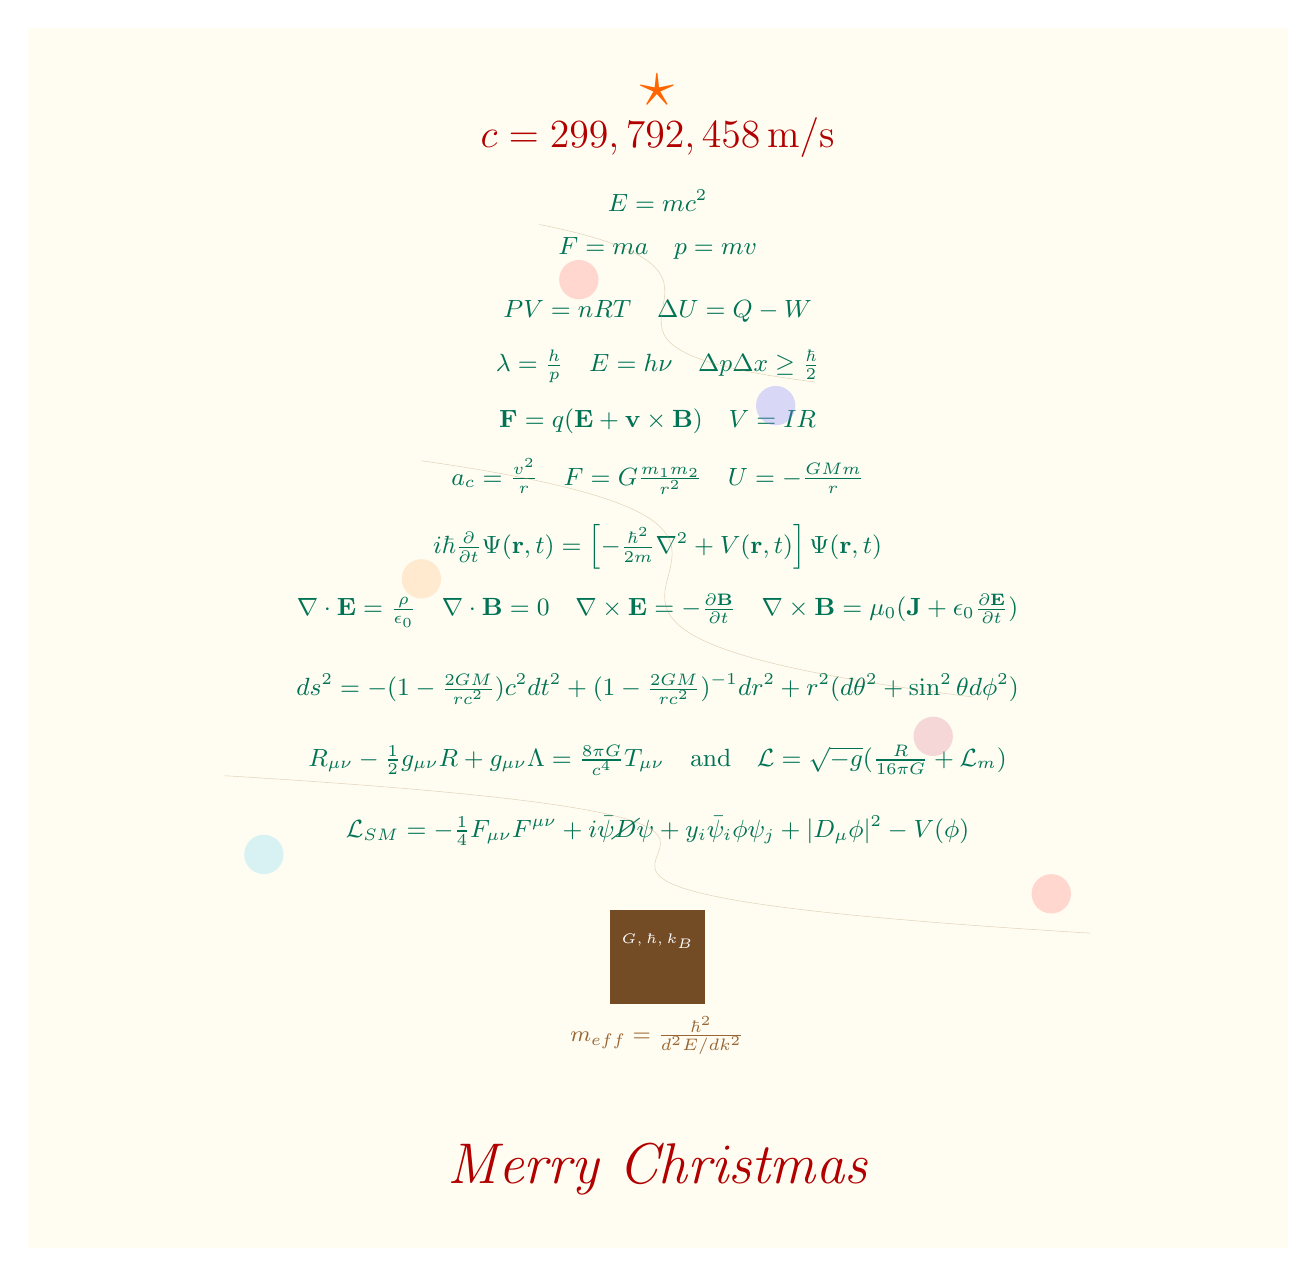
\begin{tikzpicture}
    % 背景
    \fill[bgcream] (-8,-3.5) rectangle (8,12);

    % 1. 树顶 (宇宙常数)
    \node at (0, 11.2) {\color{orange!80!red}\Huge $\star$};
    \node at (0, 10.6) {\color{red!70!black}\Large $c = 299,792,458 \, \text{m/s}$};

    % 2. 树身 (按照宽度严格递增排列)
    \begin{scope}[every node/.style={text=treegreen, font=\small, inner sep=2pt}]
        % 顶层
        \node at (0, 9.8) {$E = mc^2$};
        \node at (0, 9.2) {$F = ma \quad p = mv$};
        
        % 中层
        \node at (0, 8.4) {$PV = nRT \quad \Delta U = Q - W$};
        \node at (0, 7.7) {$\lambda = \frac{h}{p} \quad E = h\nu \quad \Delta p \Delta x \ge \frac{\hbar}{2}$};
        \node at (0, 7.0) {$\mathbf{F} = q(\mathbf{E} + \mathbf{v} \times \mathbf{B}) \quad V = IR$};
        \node at (0, 6.3) {$a_c = \frac{v^2}{r} \quad F = G \frac{m_1 m_2}{r^2} \quad U = -\frac{G M m}{r}$};
        
        % 宽层 (开始发力)
        \node at (0, 5.4) {$i\hbar \frac{\partial}{\partial t}\Psi(\mathbf{r},t) = \left[ -\frac{\hbar^2}{2m}\nabla^2 + V(\mathbf{r},t) \right] \Psi(\mathbf{r},t)$};
        \node at (0, 4.6) {$\nabla \cdot \mathbf{E} = \frac{\rho}{\epsilon_0} \quad \nabla \cdot \mathbf{B} = 0 \quad \nabla \times \mathbf{E} = -\frac{\partial \mathbf{B}}{\partial t} \quad \nabla \times \mathbf{B} = \mu_0 (\mathbf{J} + \epsilon_0 \frac{\partial \mathbf{E}}{\partial t})$};
        
        % 底部基座 (最宽处)
        \node at (0, 3.6) {$ds^2 = -(1-\frac{2GM}{rc^2})c^2dt^2 + (1-\frac{2GM}{rc^2})^{-1}dr^2 + r^2(d\theta^2 + \sin^2\theta d\phi^2)$}; % 史瓦西度规
        \node at (0, 2.7) {$R_{\mu\nu} - \frac{1}{2}g_{\mu\nu}R + g_{\mu\nu}\Lambda = \frac{8\pi G}{c^4}T_{\mu\nu} \quad \text{and} \quad \mathcal{L} = \sqrt{-g} ( \frac{R}{16\pi G} + \mathcal{L}_m )$}; % 场方程与作用量
        \node at (0, 1.8) {$\mathcal{L}_{SM} = -\frac{1}{4}F_{\mu\nu}F^{\mu\nu} + i \bar{\psi} \cancel{D}\psi + y_i \bar{\psi}_i \phi \psi_j + |D_\mu \phi|^2 - V(\phi)$}; % 标准模型拉氏量全项
    \end{scope}

    % 3. 树根 (加粗并带上物理参数)
    \fill[brown!60!black] (-0.6, -0.4) rectangle (0.6, 0.8);
    \node at (0, 0.4) {\color{white}\tiny $G, \hbar, k_B$};
    \node at (0, -0.8) {\color{brown!80!black}\footnotesize $m_{eff} = \frac{\hbar^2}{d^2E/dk^2}$};

    % 4. 装饰线 (横跨整个宽基座)
    \begin{scope}[goldline, opacity=0.4, very thin]
        \draw (-1.5, 9.5) .. controls (2, 8.8) and (-2, 8.0) .. (2, 7.5);
        \draw (-3, 6.5) .. controls (4, 5.5) and (-4, 4.5) .. (4, 3.5);
        \draw (-5.5, 2.5) .. controls (6, 1.8) and (-6, 1.2) .. (5.5, 0.5);
    \end{scope}

    % 5. 装饰波点
    \foreach \pos/\col in {(-1,8.8)/red, (1.5,7.2)/blue, (-3,5.0)/orange, (3.5,3.0)/purple, (-5,1.5)/cyan, (5,1.0)/red}
        \fill[\col!50, opacity=0.3] \pos circle (0.25);

    % 6. 底部祝福
    \node at (0, -2.5) {\color{red!70!black}\huge \it Merry Christmas};

\end{tikzpicture}
\end{document}